% Author: Dr. Matthias Jung, DL9MJ
% Year: 2020
% TB601
\documentclass[convert = false, border=5pt, varwidth]{standalone}
\usepackage{fontspec}
\setmainfont{Roboto}
\usepackage[siunitx, straightvoltages, europeanresistors, european inductor]{circuitikzgit}
\usepackage{tikz}


\usepackage{tikz,pgfplots}
\usetikzlibrary{arrows}

\usepackage{amsmath}
\usepackage{unicode-math}
\setmathfont{Fira Math}
\setmathfont[range=up]{Roboto}
\setmathfont[range=it]{Roboto-Italic}
\setmathfont[range=\int]{Fira Math}
\usepackage[euler]{textgreek}

\begin{document}

\pgfplotsset{
  every axis plot/.append style={line width=0.8pt},
}

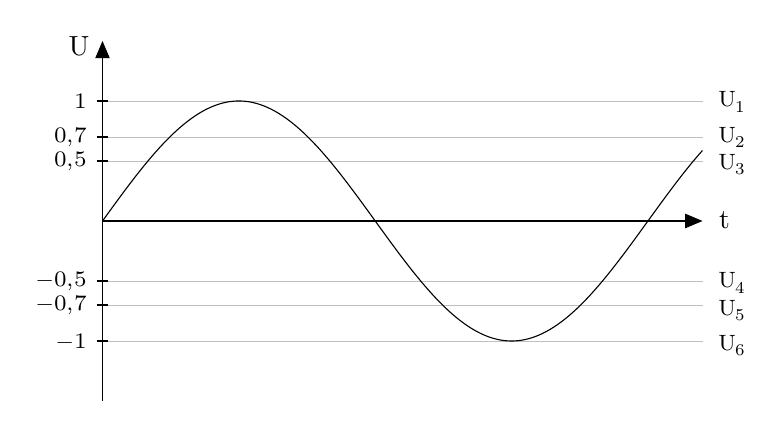
\begin{tikzpicture}
    \draw (-0.3,4.5) node[]{U};
    %\draw ( 7.9,2.3) node[]{$\omega$t};
    \draw ( 7.9,2.3) node[]{t};
    \draw (   8,3.0) node[]{\footnotesize{$\mathrm{U}_3$}};
    \draw (   8,3.35) node[]{\footnotesize{$\mathrm{U}_2$}};
    \draw (   8,3.8) node[]{\footnotesize{$\mathrm{U}_1$}};
    \draw (   8,0.7) node[]{\footnotesize{$\mathrm{U}_6$}};
    \draw (   8,1.15) node[]{\footnotesize{$\mathrm{U}_5$}};
    \draw (   8,1.5) node[]{\footnotesize{$\mathrm{U}_4$}};
    \begin{axis}[%
        /pgf/number format/1000 sep={ },
        /pgf/number format/use comma,        
        axis lines=middle,
        axis line style={-triangle 45},
        width=3in,
        height=1.8in,
        scale only axis,
        %yticklabel=\empty,
        ytick={-1,-0.7,-0.5,0,0.5,0.7,1},
        grid=major,
        grid style={line width=.1pt, draw=gray!10},
        major grid style={line width=.2pt,draw=gray!50},
        xticklabel=\empty,
        %ticks=none,
        xtick style={draw=none},
        xmin=0,
        xmax=2.2*pi,
        ymin=-1.5,
        ymax=1.5,
        xmajorgrids=false,
        label style={font=\small},
        tick label style={font=\footnotesize},
        every major tick/.append style={thick, black}
    ]
    \addplot[samples=500,domain=0:2.2*pi,smooth,black] {sin(deg(x))}; 
\end{axis}
\end{tikzpicture}%
\end{document}
